\documentclass{beamer}
\usepackage[utf8]{inputenc}

\usetheme{Madrid}
\usecolortheme{default}
\usepackage{amsmath,amssymb,amsfonts,amsthm}
\usepackage{txfonts}
\usepackage{tkz-euclide}
\usepackage{listings}
\usepackage{adjustbox}
\usepackage{array}
\usepackage{tabularx}
\usepackage{gvv}
\usepackage{lmodern}
\usepackage{circuitikz}
\usepackage{tikz}
\usepackage{graphicx}
\usepackage{amsmath}

\setbeamertemplate{page number in head/foot}[totalframenumber]

\usepackage{tcolorbox}
\tcbuselibrary{minted,breakable,xparse,skins}



\definecolor{bg}{gray}{0.95}
\DeclareTCBListing{mintedbox}{O{}m!O{}}{%
  breakable=true,
  listing engine=minted,
  listing only,
  minted language=#2,
  minted style=default,
  minted options={%
    linenos,
    gobble=0,
    breaklines=true,
    breakafter=,,
    fontsize=\small,
    numbersep=8pt,
    #1},
  boxsep=0pt,
  left skip=0pt,
  right skip=0pt,
  left=25pt,
  right=0pt,
  top=3pt,
  bottom=3pt,
  arc=5pt,
  leftrule=0pt,
  rightrule=0pt,
  bottomrule=2pt,
  toprule=2pt,
  colback=bg,
  colframe=orange!70,
  enhanced,
  overlay={%
    \begin{tcbclipinterior}
    \fill[orange!20!white] (frame.south west) rectangle ([xshift=20pt]frame.north west);
    \end{tcbclipinterior}},
  #3,
}
\lstset{
    language=C,
    basicstyle=\ttfamily\small,
    keywordstyle=\color{blue},
    stringstyle=\color{orange},
    commentstyle=\color{green!60!black},
    numbers=left,
    numberstyle=\tiny\color{gray},
    breaklines=true,
    showstringspaces=false,
}


\title 
{2.6.32}
\date{September 08,2025}


\author 
{Abhiram Reddy-AI25BTECH11021}



\begin{document}


\frame{\titlepage}
%------------------------------------
\begin{frame}{Problem Statement}
Find the area of the triangle whose vertices are
\[
(1, -1), \quad (-4, 6), \quad (-3, 5).
\]
\end{frame}

\begin{frame}{Step 1: Define the vertices as vectors}
\[
A = \begin{pmatrix} 1 \\ -1 \end{pmatrix}, \quad
B = \begin{pmatrix} -4 \\ 6 \end{pmatrix}, \quad
C = \begin{pmatrix} -3 \\ 5 \end{pmatrix}
\]
\end{frame}

\begin{frame}{Step 2: Calculate the vectors \( A - B \) and \( B - C \)}
\[
A - B = \begin{pmatrix} 1 \\ -1 \end{pmatrix} - \begin{pmatrix} -4 \\ 6 \end{pmatrix} 
= \begin{pmatrix} 5 \\ -7 \end{pmatrix}
\]

\[
B - C = \begin{pmatrix} -4 \\ 6 \end{pmatrix} - \begin{pmatrix} -3 \\ 5 \end{pmatrix} 
= \begin{pmatrix} -1 \\ 1 \end{pmatrix}
\]
\end{frame}

\begin{frame}{Step 3: Calculate the 2D cross product magnitude}
For vectors \(\mathbf{u} = \begin{pmatrix} u_1 \\ u_2 \end{pmatrix}\) and \(\mathbf{v} = \begin{pmatrix} v_1 \\ v_2 \end{pmatrix}\), the 2D cross product is
\[
\mathbf{u} \times \mathbf{v} = u_1 v_2 - u_2 v_1.
\]

Applying this,
\[
(A-B) \times (B-C) = 5 \times 1 - (-7) \times (-1) = 5 - 7 = -2
\]

\[
\Rightarrow \| (A-B) \times (B-C) \| = 2
\]
\end{frame}

\begin{frame}{Step 4: Calculate the area of the triangle}
\[
ar(ABC) = \frac{1}{2} \times \| (A-B) \times (B-C) \| = \frac{1}{2} \times 2 = 1
\]

\[
\boxed{ar(ABC) = 1 \text{ square unit}}
\]
\end{frame}

% C code split in two frames
\begin{frame}[fragile]{C Code (Part 1)}
\begin{lstlisting}[language=C]
#include <stdio.h>
#include <math.h>  // For fabs()

double crossProduct(double u1, double u2, double v1, double v2) {
    return u1 * v2 - u2 * v1;
}

int main() {
    double Ax = 1, Ay = -1;
    double Bx = -4, By = 6;
    double Cx = -3, Cy = 5;
\end{lstlisting}
\end{frame}

\begin{frame}[fragile]{C Code (Part 2)}
\begin{lstlisting}[language=C]
    double ABx = Ax - Bx;
    double ABy = Ay - By;
    double BCx = Bx - Cx;
    double BCy = By - Cy;

    double cross = crossProduct(ABx, ABy, BCx, BCy);
    double area = 0.5 * fabs(cross);

    printf("Area of triangle ABC = %.2f square units\n", area);
    return 0;
}
\end{lstlisting}
\end{frame}

% Python code split in two frames
\begin{frame}[fragile]{Python Code (Part 1)}
\begin{lstlisting}[language=Python]
import matplotlib.pyplot as plt

A = (1, -1)
B = (-4, 6)
C = (-3, 5)

x_coords = [A[0], B[0], C[0], A[0]]
y_coords = [A[1], B[1], C[1], A[1]]
\end{lstlisting}
\end{frame}

\begin{frame}[fragile]{Python Code (Part 2)}
\begin{lstlisting}[language=Python]
plt.figure()
plt.plot(x_coords, y_coords, 'b-', marker='o')

plt.text(A[0], A[1], 'A', fontsize=12, ha='right')
plt.text(B[0], B[1], 'B', fontsize=12, ha='right')
plt.text(C[0], C[1], 'C', fontsize=12, ha='right')

plt.gca().set_aspect('equal', adjustable='box')
plt.grid(True)

plt.title('Triangle ABC')
plt.xlabel('x')
plt.ylabel('y')

plt.savefig('python_plot.png')
plt.show()
\end{lstlisting}
\end{frame}





\begin{frame}{Plot}
    \centering
    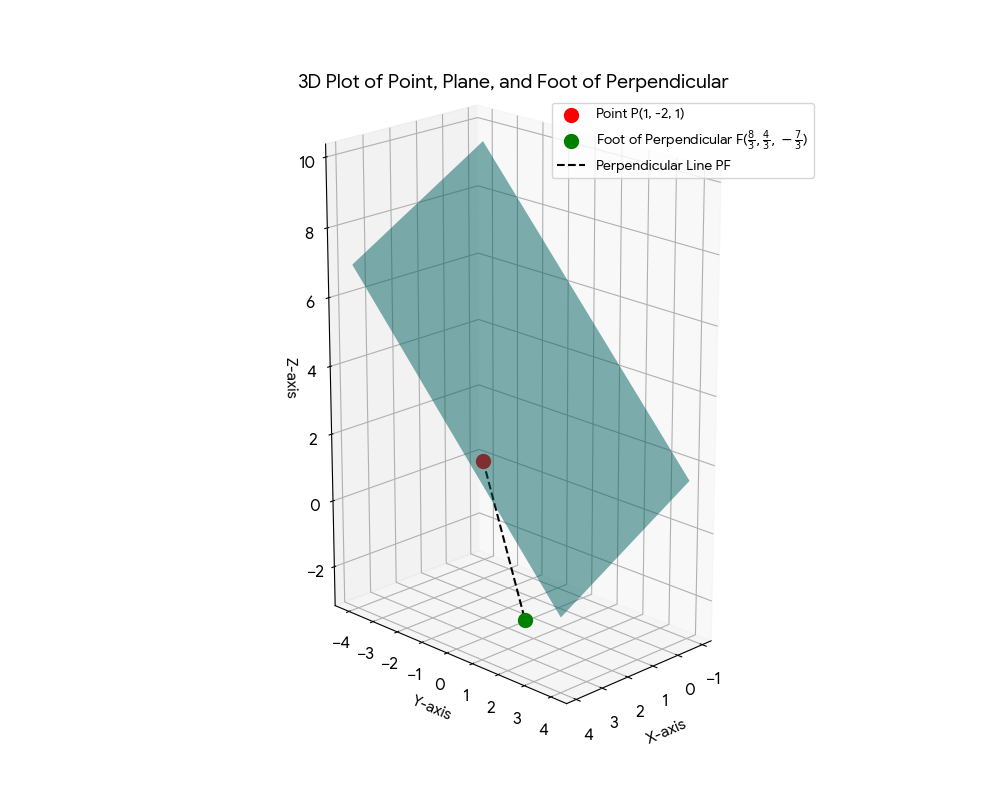
\includegraphics[width=\columnwidth, height=0.8\textheight, keepaspectratio]{figs/python_plot.png}     
\end{frame}


\end{document}